


\colorlet{tp}{teal!50!purple}



\AddToShipoutPictureFG{


\ifnum\value{page}=2{
\AtTextLowerLeft{\raisebox{522pt}{

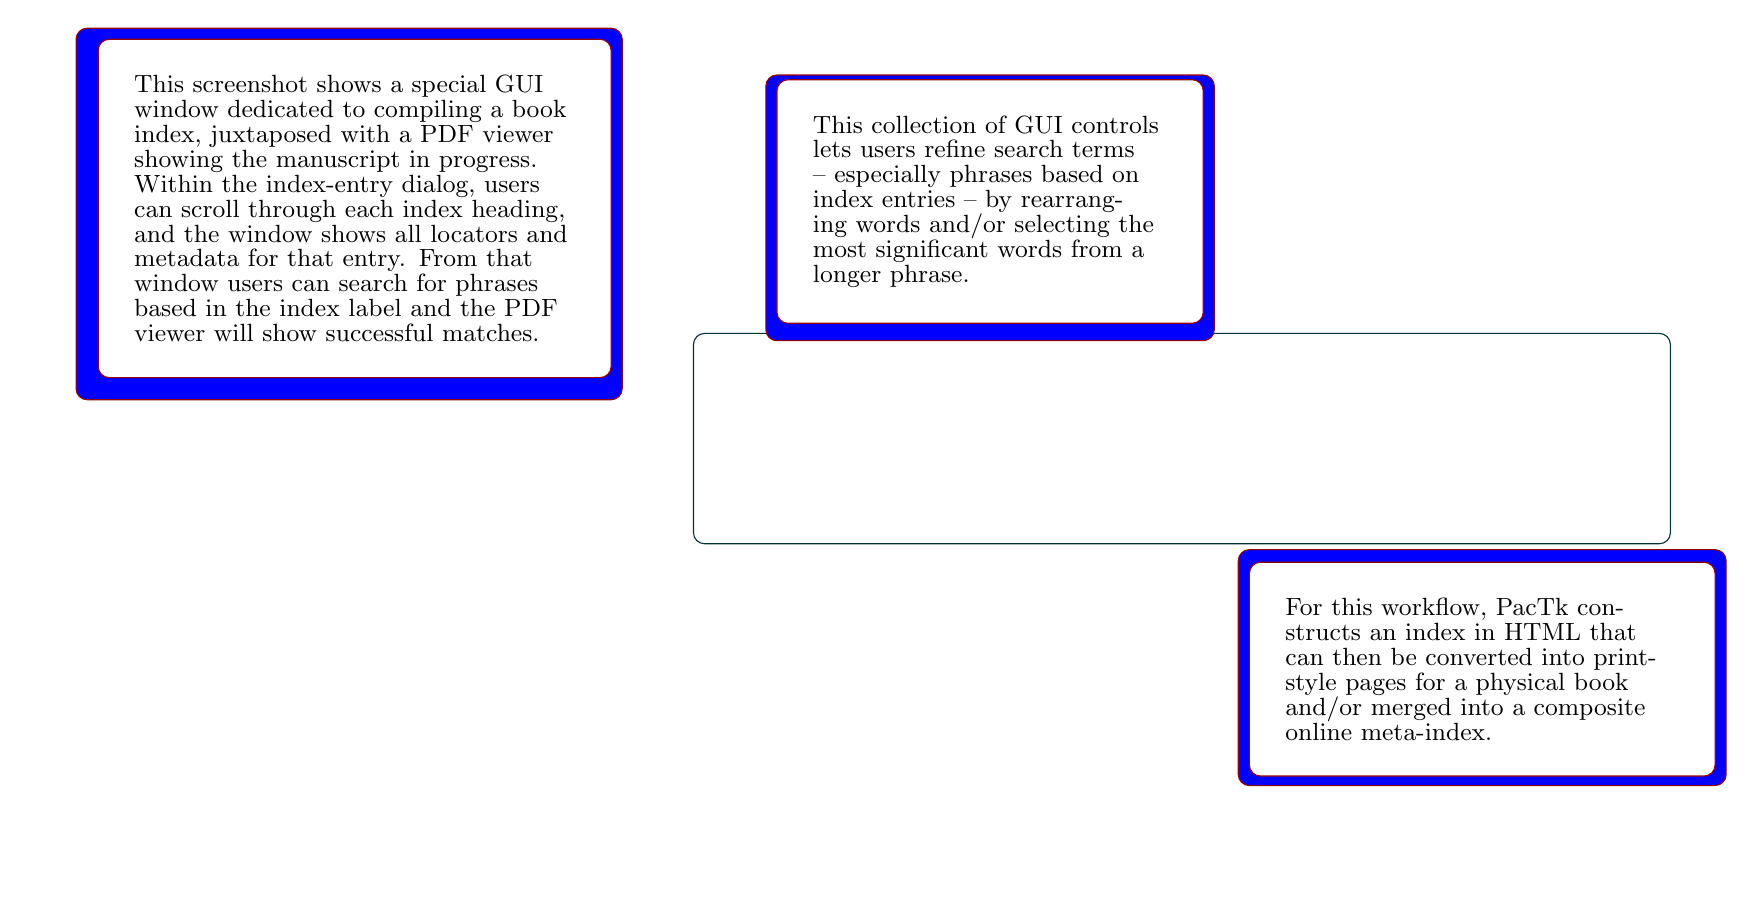
\begin{tikzpicture}

\node at (0,0) [text=white] {X};

%\draw (.6,4.3) circle  (6pt) [xscale=1.4];
%\draw (1,0) circle (6pt);

%\node [draw, circle, minimum size=8pt,xscale=2.7, 
%draw=teal!40!black] (s1) at (.63,4.24) {};


%\node [draw, circle, minimum size=8pt,xscale=2.7, 
%draw=teal!40!black] (n1) at (.93,11.29) {};


%\node [draw, rectangle, minimum width=40pt, minimum height=13pt, 
%anchor = south west, rounded corners,
%draw=teal!40!black] (s2) at (4.78,3.2) {};


%\node [draw, rectangle, minimum width=40pt, minimum height=13pt, 
%anchor = south west, rounded corners,
%draw=teal!40!black] (n2) at (9.3,10.78) {};


%\node [draw, rectangle, minimum width=40pt, minimum height=13pt, 
%anchor = south west, rounded corners,
%draw=teal!40!black] (n3) at (13.7,10.78) {};




%\node [draw, rectangle, minimum width=40pt, minimum height=13pt, 
%anchor = south west, rounded corners,
%draw=teal!40!black] (s3) at (18.65,4.53) {};



\node [draw=red!60!black, fill=blue, anchor = south west, rounded corners,
text width=5.6cm, inner sep=19pt, xshift=-8pt, yshift=-8pt, font={\fontsize{9}{9}\selectfont}] (ltext)
 at (.64, 6.1) {{This screenshot shows a special GUI window dedicated to 
compiling a book index, juxtaposed with a PDF viewer showing the 
manuscript in progress.  Within the index-entry dialog, users can scroll 
through each index heading, and the window shows all locators and metadata 
for that entry.  From that window users can search for phrases based 
in the index label and the PDF viewer will show successful matches.}
};


\node [draw=red!60!black, fill=white, anchor = south west, rounded corners,
text width=5.6cm, inner sep=13pt, font={\fontsize{9}{9}\selectfont}] (ltext-outer)
 at (.64, 6.1) {This screenshot shows a special GUI window dedicated to 
compiling a book index, juxtaposed with a PDF viewer showing the 
manuscript in progress.  Within the index-entry dialog, users can scroll 
through each index heading, and the window shows all locators and metadata 
for that entry.  From that window users can search for phrases based 
in the index label and the PDF viewer will show successful matches.
};


%\draw (ltext) -- (s1);
%



%\node [draw, rectangle, minimum width=340pt, minimum height=40pt, 
%anchor = south west, rounded corners,
%draw=teal!40!black] at (6.8,.76) {};


\node [draw=red!60!black, fill=blue, anchor = south west, rounded corners,
text width=5cm, inner sep=17pt, xshift=-8pt, yshift=-8pt, font={\fontsize{9}{9}\selectfont}] (ltext)
 at (15.4, 1.2) {{For this workflow, PacTk constructs an index in HTML that can then 
be converted into print-style pages for a physical book and/or merged into a 
composite online meta-index.
}
};


\node [draw=red!60!black, fill=white, anchor = south west, rounded corners,
text width=5cm, inner sep=13pt, font={\fontsize{9}{9}\selectfont}] (ltext-outer)
 at (15.26, 1.04) {For this workflow, PacTk constructs an index in HTML that can then 
be converted into print-style pages for a physical book and/or merged into a 
composite online meta-index.
};





\node [draw, rectangle, minimum width=353pt, minimum height=76pt, 
anchor = south west, rounded corners,
draw=teal!40!black] at (8.2,3.99) {};


\node [draw=red!60!black, fill=blue, anchor = south west, rounded corners,
text width=4.5cm, inner sep=17pt, xshift=-8pt, yshift=-8pt, font={\fontsize{9}{9}\selectfont}] (ltext)
 at (9.4, 6.85) {{This collection of GUI controls lets users refine search terms -- especially 
phrases based on index entries --  
by rearranging words and/or selecting the most significant words from a 
longer phrase.
} 
};


\node [draw=red!60!black, fill=white, anchor = south west, rounded corners,
text width=4.5cm, inner sep=13pt, font={\fontsize{9}{9}\selectfont}] (ltext-outer)
 at (9.26, 6.79) {This collection of GUI controls lets users refine search terms -- especially 
phrases based on index entries --   
by rearranging words and/or selecting the most significant words from a 
longer phrase.
};





\end{tikzpicture}


}}


}\fi





\ifnum\value{page}=3{
\AtTextLowerLeft{\raisebox{522pt}{

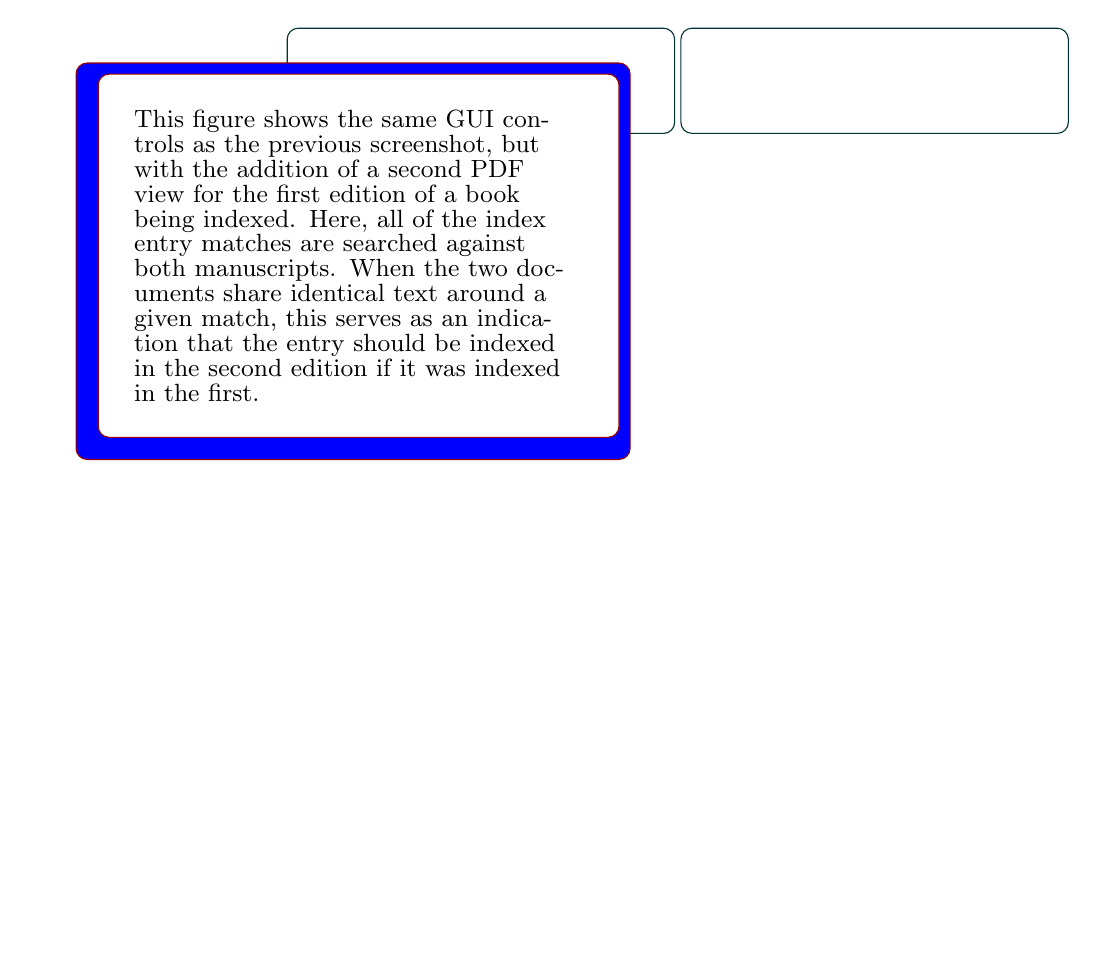
\begin{tikzpicture}

\node at (0,0) [text=white] {X};

%\draw (.6,4.3) circle  (6pt) [xscale=1.4];
%\draw (1,0) circle (6pt);

%\node [draw, circle, minimum size=8pt,xscale=2.7, 
%draw=teal!40!black] (s1) at (.63,4.24) {};


%\node [draw, circle, minimum size=8pt,xscale=2.7, 
%draw=teal!40!black] (n1) at (.93,11.29) {};


%\node [draw, rectangle, minimum width=40pt, minimum height=13pt, 
%anchor = south west, rounded corners,
%draw=teal!40!black] (s2) at (4.78,3.2) {};


%\node [draw, rectangle, minimum width=40pt, minimum height=13pt, 
%anchor = south west, rounded corners,
%draw=teal!40!black] (n2) at (9.3,10.78) {};


%\node [draw, rectangle, minimum width=40pt, minimum height=13pt, 
%anchor = south west, rounded corners,
%draw=teal!40!black] (n3) at (13.7,10.78) {};




%\node [draw, rectangle, minimum width=40pt, minimum height=13pt, 
%anchor = south west, rounded corners,
%draw=teal!40!black] (s3) at (18.65,4.53) {};



\node [draw, rectangle, minimum width=140pt, minimum height=38pt, 
anchor = south west, rounded corners,
draw=teal!40!black] at (3.04,9.96) {};

\node [draw, rectangle, minimum width=140pt, minimum height=38pt, 
anchor = south west, rounded corners,
draw=teal!40!black] at (8.04,9.96) {};



\node [draw=red!60!black, fill=blue, anchor = south west, rounded corners,
text width=5.7cm, inner sep=19pt, xshift=-8pt, yshift=-8pt, font={\fontsize{9}{9}\selectfont}] (ltext)
 at (.64, 6.1) {{This figure shows the same GUI controls as the previous 
screenshot, but with the addition of a second PDF view for the first 
edition of a book being indexed.  Here, all of the index entry 
matches are searched against both manuscripts.  When the  
two documents share identical text around a given match, this 
serves as an indication that the entry should be indexed in 
the second edition if it was indexed in the first.}
};


\node [draw=red!60!black, fill=white, anchor = south west, rounded corners,
text width=5.7cm, inner sep=13pt, font={\fontsize{9}{9}\selectfont}] (ltext-outer)
 at (.64, 6.1) {This figure shows the same GUI controls as the previous 
screenshot, but with the addition of a second PDF view for the first 
edition of a book being indexed.  Here, all of the index entry 
matches are searched against both manuscripts.  When the  
two documents share identical text around a given match, this 
serves as an indication that the entry should be indexed in 
the second edition if it was indexed in the first.
};


%\draw (ltext) -- (s1);
%



%\node [draw, rectangle, minimum width=340pt, minimum height=40pt, 
%anchor = south west, rounded corners,
%draw=teal!40!black] at (6.8,.76) {};







\end{tikzpicture}


}}


}\fi






\ifnum\value{page}=8{
\AtTextLowerLeft{\raisebox{499pt}{

\begin{tikzpicture}

\node at (0,0) [text=white] {X};


\node [draw=red!60!black, fill=blue, anchor = north west, rounded corners,
text width=14.64cm, inner sep=17pt, xshift=-8pt, yshift=-8pt, font={\fontsize{9}{9}\selectfont}] (ltext)
(s1) at (3.52, 11.64) {{
PacTk enables fine-grained metadata to be embedded in documents, representing 
PDF page coordinates for sentence and paragraph start/end points, as well as 
locations for keywords, proper names (and other Named Entities), 
figure illustrations, and other publication landmarks.   
}
};


\node [draw=red!60!black, fill=white, anchor = north west, rounded corners,
text width=14.64cm, inner sep=13pt, font={\fontsize{9}{9}\selectfont}] (ltext-inner)
 at (3.43, 11.2) {
PacTk enables fine-grained metadata to be embedded in documents, representing 
PDF page coordinates for sentence and paragraph start/end points, as well as 
locations for keywords, proper names (and other Named Entities), 
figure illustrations, and other publication landmarks.
};





\node [draw=red!60!black, fill=blue, anchor = north west, rounded corners,
text width=7.64cm, inner sep=17pt, xshift=-8pt, yshift=-8pt, font={\fontsize{9}{9}\selectfont}] 
(stext) at (.3, 2.64) {{
With a conformant PDF viewer, users can examine PacTk metadata directly, which 
can be useful for programmers intending to develop text-mining algorithms.  
}
};


\node [draw=red!60!black, fill=white, anchor = north west, rounded corners,
text width=7.64cm, inner sep=13pt, font={\fontsize{9}{9}\selectfont}] (stext-inner)
 at (.25, 2.2) {
With a conformant PDF viewer, users can examine PacTk metadata directly, which 
can be useful for programmers intending to develop text-mining algorithms.  
};


\draw  [->,>=stealth', line width=4pt, draw=tp!50] ([yshift=48pt, xshift=148] stext.east) to 
  [bend left=20]  ([yshift=-22, xshift=2] stext.east) ;


\draw  [->,>=stealth', line width=4pt, draw=tp!50] ([yshift=28pt, xshift=-18] stext.north) to 
  [bend left=20]  ([yshift=2, xshift=2] stext.north) ;


\draw  [->,>=stealth', line width=4pt, draw=tp!30!magenta] ([yshift=89pt, xshift=179] stext.north) to 
  [bend left=20]  ([yshift=128pt, xshift=274] stext.north) ;


\end{tikzpicture}
}}

}\fi






\ifnum\value{page}=4{
\AtTextLowerLeft{\raisebox{21pt}{

\begin{tikzpicture}

\node at (0,0) [text=white] {X};

\begin{scope}[transform canvas={scale=0.6, shift={(21.6,20.5)}},overlay]

\draw [rotate=20.9245, fill=white] (-1.5pt, 0pt) -- ++(up:5pt) -- ++(-5pt, -2pt) -- ++(6.5pt, 17pt)
                      -- ++(6.5pt, -17pt) -- ++(-5pt, 2pt) -- ++(down:5pt) -- cycle;

\end{scope}


\definecolor{fillc}{RGB}{130, 89, 68}

\node [draw=fillc!80!cyan, fill=fillc!50!red, anchor = north west, rounded corners,
text width=7.64cm, inner sep=17pt, xshift=-8pt, yshift=-8pt, font={\fontsize{9}{9}\selectfont}] (ltext)
at (3.52, 10.54) {{A meta-index search routed from a local PDF file through a 
web portal, resulting in the retrieval of another 
book title in the same series, or potentially anywhere within 
the publisher's repository.  The new book 
is then retrieved as a PDF file and opened 
to the relevant page-match and can be seen side-by-side, 
thus keeping the reader's attention 
instead of opening a new browsing session.}
};


\node [draw=fillc!80!cyan, fill=white, anchor = north west, rounded corners,
text width=7.64cm, inner sep=13pt, font={\fontsize{9}{9}\selectfont}] (ltext-inner)
 at (3.37, 10.1) {
A meta-index search routed from a local PDF file through a 
web portal, resulting in the retrieval of another 
book title in the same series, or potentially anywhere within 
the publisher's repository.  The new book 
is then retrieved as a PDF file and opened 
to the relevant page-match and can be seen side-by-side, 
thus keeping the reader's attention 
instead of opening a new browsing session.
};




\node [draw=fillc!80!cyan, fill=fillc!50!red, anchor = north west, rounded corners,
text width=5.64cm, inner sep=11pt, xshift=-8pt, yshift=-8pt, font={\fontsize{9}{9}\selectfont}] (stext)
at (13.52, 4.54) {{Evan Stark, \textit{Coercive Control:
How Men Entrap Women in Personal Life} (Oxford University Press, 2023) p. 69.}
};


\node [draw=fillc!80!cyan, fill=white, anchor = north west, rounded corners,
text width=5.64cm, inner sep=8pt, font={\fontsize{9}{9}\selectfont}] (s)
 at (13.37, 4.1) {Evan Stark, \textit{Coercive Control:
How Men Entrap Women in Personal Life} (Oxford University Press, 2023), p. 69.
};



\draw  [->,>=stealth', line width=4pt, draw=tp!50] ([yshift=84pt, xshift=-77pt] ltext.north west) to 
   ([yshift=163pt, xshift=-50pt] ltext.north east) ;



\draw  [->,>=stealth', line width=4pt, draw=tp!50] 
   ([yshift=273pt, xshift=64pt] ltext.north east) to 
   ([yshift=53pt, xshift=95pt] ltext.north east) ;




\end{tikzpicture}
}}

}\fi





\ifnum\value{page}=5{
\AtTextLowerLeft{\raisebox{551pt}{

\begin{tikzpicture}

\node at (0,0) [text=white] {X};



\node[shape=circle,draw=circ!40,line width=4pt, text=circ,fill=red!4,text centered,text width=8pt,inner sep=4pt] at (2.7,10) {1};
\node[shape=circle,draw=circ,line width=1pt, text=circ,fill=red!4,text centered,text width=8pt,inner sep=4pt] at (2.7,10) {1};


\node[shape=circle,draw=circ!40,line width=4pt, text=circ,fill=red!4,text centered,text width=8pt,inner sep=4pt] at (11.1,4.3) {2};
\node[shape=circle,draw=circ,line width=1pt, text=circ,fill=red!4,text centered,text width=8pt,inner sep=4pt] at (11.1,4.3) {2};



\node[shape=circle,draw=circ!40,line width=4pt, text=circ,fill=red!4,text centered,text width=8pt,inner sep=4pt] at (2.8,3.5) {3};
\node[shape=circle,draw=circ,line width=1pt, text=circ,fill=red!4,text centered,text width=8pt,inner sep=4pt] at (2.8,3.5) {3};



\colorlet{bgray}{blue!30!gray}
\colorlet{ou}{purple!60!red}
\colorlet{in}{orange!60!black}


\node [draw=ou!30, fill=bgray!49, anchor = south west, rounded corners,
text width=7.5cm, inner sep=17pt, xshift=-8pt, yshift=-8pt, font={\fontsize{9}{9}\selectfont}] (ltext)
(s1) at (3.9, .8) {{Paragraphs where the matches are located 
are also highlighted at their start and end points (\tcircledb{2} and \tcircledb{3}).
}
};


\node [draw=in!60, fill=white, anchor = south west, rounded corners,
text width=7.5cm, inner sep=13pt, font={\fontsize{9}{9}\selectfont}] (ltext-outer)
 at (3.83, .7) {Paragraphs where the matches are located 
are also highlighted at their start and end points (\tcircledb{2} and \tcircledb{3}).
};


\node [draw=ou!30, fill=bgray!49, anchor = south west, rounded corners,
text width=11.8cm, inner sep=17pt, xshift=-8pt, yshift=-8pt, font={\fontsize{9}{9}\selectfont}] (ltext)
(s1) at (8.4, 5.9) {{Using highlights to indicate index entry locators.  
This paragraph shows highlights applied after a user selects the 
main entry (Harold Garfinkel) from the index.  For convenient 
browsing, search-matching terms are shown on a side-bar, alongside 
a clickable arrow allowing users to browse to the next match 
from the index (\tcircledb{1}).  Related entries identified via \textit{see also} 
or subentry data from the index are also highlighted.
}
};


\node [draw=in!60, fill=white, anchor = south west, rounded corners,
text width=11.8cm, inner sep=13pt, font={\fontsize{9}{9}\selectfont}] (ltext-outer)
 at (8.25, 5.7) {Using highlights to indicate index entry locators.  
This paragraph shows highlights applied after a user selects the 
main entry (Harold Garfinkel) from the index.  For convenient 
browsing, search-matching terms are shown on a side-bar, alongside 
a clickable arrow allowing users to browse to the next match 
from the index (\tcircledb{1}).  Related entries identified via \textit{see also} 
or subentry data from the index are also highlighted.
};




\end{tikzpicture}
}}

}\fi







\ifnum\value{page}=6{
\AtTextLowerLeft{\raisebox{599pt}{

\begin{tikzpicture}

\node at (0,0) [text=white] {X};


\definecolor{clrmcMidr}{RGB}{53, 143, 222}
\definecolor{clrmcMid}{RGB}{165, 10, 18}
\definecolor{cdotchere}{RGB}{186, 60, 6}
\definecolor{cdotcherer}{RGB}{53, 214, 222}

\definecolor{clrmcrAlt}{RGB}{130, 89, 68}

\definecolor{clrmcr}{RGB}{0, 148, 123}
\definecolor{clrmcrr}{RGB}{7, 165, 232}


\newcommand{\clrmrAltFmt}[2]{%
\textcolor{clrmcrr}{%
\raisebox{-1.5pt}{\resizebox{4pt}{5pt}{\ensuremath{\Rsh}}}}%
\textcolor{clrmcr}{%
{\fontsize{8}{6}\selectfont{#1}}}%
\hspace{.5pt}\raisebox{.5pt}{%
\textcolor{clrmcrAlt}{%
{\fontsize{7}{6}\selectfont{#2}}}}%
}


\definecolor{cdotc}{RGB}{186, 99, 11}


\newcommand{\clrmAltDot}{%
\resizebox{1.5pt}{1.5pt}{\textbullet}}


\newcommand{\clrmAltFmt}[1]{%
\textcolor{clrmcMid}{%
\raisebox{.5pt}{%\resizebox{6pt}{.5pt}{%
\textcolor{cdotc}{\clrmAltDot{}\hspace{1pt}%
\clrmAltDot{}\hspace{1pt}\clrmAltDot{}%
%\ensuremath{\blacksquare}
}%
}%
{\fontsize{8}{6}\selectfont{#1}}}}


\definecolor{margin}{RGB}{133, 20, 12}


\node [draw=red!60!black, fill=blue, anchor = south west, rounded corners,
text width=8.2cm, inner sep=17pt, xshift=-8pt, yshift=-8pt, font={\fontsize{9}{9}\selectfont}] (ltext)
(s1) at (1.4, 5.1) {{Para Ids for this PacTk document 
are color-coded, with outlined numbers (42., etc.) for ordinary 
paragraphs, roman\\numerals (\textcolor{clrmcMid!20!gray}{$i$}, 
\textcolor{clrmcMid!20!gray}{$ii$}) for block quotes, 
and English letters (\textcolor{cdotchere}{a}, \textcolor{cdotchere}{b}, etc.) for 
continuations after quotes or enumerations.  Special formats 
are also applied to the portion of paragraphs at the\\top 
of a page/column (near the bottom of the screenshot, 
these styles are visible in the continuation 
45 and \clrmrAltFmt{48}{a} symbols).\vspace*{-5pt}
}
};


\node [draw=red!60!black, fill=white, anchor = south west, rounded corners,
text width=8.2cm, inner sep=13pt, font={\fontsize{9}{9}\selectfont}] (ltext-outer)
 at (1.33, 5) {Para Ids for this PacTk document 
are color-coded, with outlined numbers (\textcolor{white}{42.}, etc.) for ordinary 
paragraphs, roman\\numerals (\textcolor{clrmcMid!20!gray}{$i$}, 
\textcolor{clrmcMid!20!gray}{$ii$}) for block quotes, 
and English letters (\textcolor{cdotchere}{a}, \textcolor{cdotchere}{b}, etc.) for 
continuations after quotes or enumerations.  Special formats 
are also applied to the portion of paragraphs at the\\top 
of a page/column (near the bottom of the screenshot, 
these styles are visible in the continuation 
\clrmAltFmt{45} and \clrmrAltFmt{48}{a} symbols).\vspace*{-4pt}
};

\begin{scope}[transform canvas={scale=.6}]
%\begin{scope}[xscale=6]

 \node[shape=regular polygon, regular polygon sides = 8,
fill = margin!10, inner sep=1pt] at (6.66, 11.78) (char)
{42};

 \node[shape=regular polygon, regular polygon sides = 8,
fill opacity=0, line width=2pt, draw=yellow!5, inner sep=1pt] 
at (char) 
%top color=white, bottom color=blggr!6,
%fill opacity=1, yscale=.7, shape border rotate=39,
%inner sep=6.5pt, shading angle=90,label={}] (bk) 
{\phantom{42}};


\end{scope}


\begin{scope}[shift={(190pt,-40pt)}]

\node [draw=purple!60!red, fill=white, anchor = south west, rounded corners,
text width=4.6cm, inner sep=14.5pt, font={\fontsize{9}{9}\selectfont}] (ltext-lower)
 at (2.28, 0.28) {The document's index incorporates the same paragraph-id 
symbols\\as printed on the margins, to\\create clickable locators 
targeted at individual paragraphs and their subdivisions. 
};


\node [draw=orange!60!black, fill=white, anchor = south west, rounded corners,
text width=4.6cm, inner sep=13pt, font={\fontsize{9}{9}\selectfont}] (ltext-lower)
 at (2.33, 0.34) {The document's index incorporates the same paragraph-id 
symbols\\as printed on the margins, to\\create clickable locators 
targeted at individual paragraphs and their subdivisions.};

\end{scope}


\end{tikzpicture}
}}

}\fi





\ifnum\value{page}=6{
\AtTextLowerLeft{\raisebox{-108pt}{

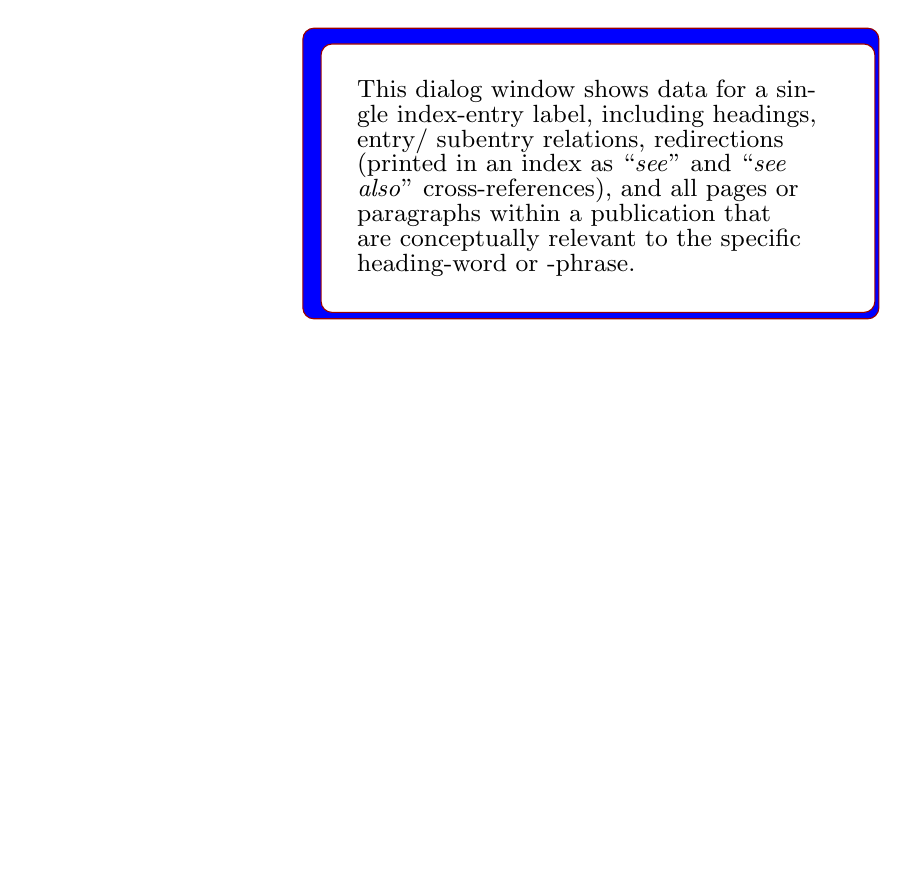
\begin{tikzpicture}

\node at (0,0) [text=white] {X};


\node [draw=red!60!black, fill=blue, anchor = south west, rounded corners,
text width=6.12cm, inner sep=17pt, xshift=-8pt, yshift=-8pt, font={\fontsize{9}{9}\selectfont}] (ltext)
(s1) at (3.52, 6.7) {{
This dialog window shows data for a single index-entry label, including entry/ subentry 
relations, redirections (printed in an index as ``\textit{see}'' 
and ``\textit{see also}'' cross-references), 
headings, and all pages or paragraphs within a publication that 
are conceptually relevant to the specific heading-word or -phrase.
}
};


\node [draw=red!60!black, fill=white, anchor = south west, rounded corners,
text width=6.12cm, inner sep=13pt, font={\fontsize{9}{9}\selectfont}] (ltext-outer)
 at (3.47, 6.5) {
This dialog window shows data for a single index-entry label, including \makebox{headings}, 
entry/ subentry 
relations, redirections (printed in an index as ``\textit{see}'' 
and ``\textit{see also}'' cross-references), 
and all pages or paragraphs within a publication that 
are conceptually relevant to the specific heading-word or -phrase.
};

\end{tikzpicture}
}}

}\fi





\ifnum\value{page}=7{
\AtTextLowerLeft{\raisebox{471pt}{

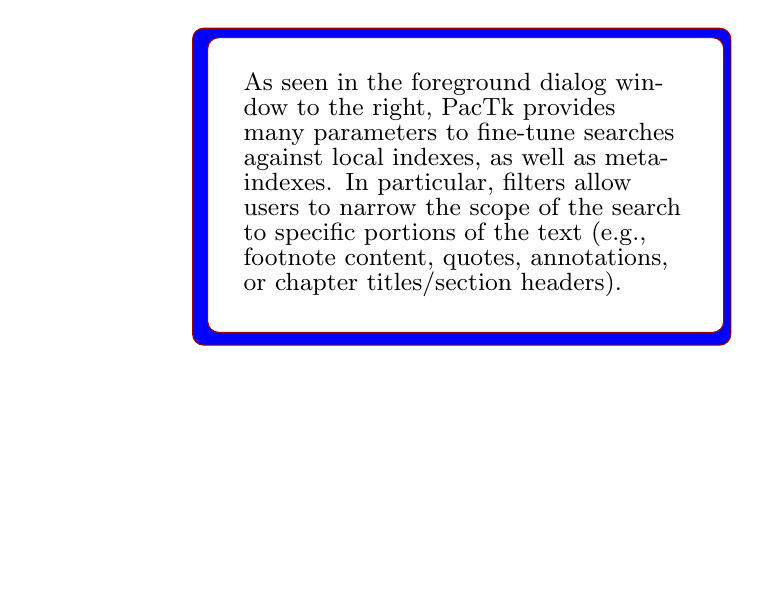
\begin{tikzpicture}

\node at (0,0) [text=white] {X};




\node [draw=red!60!black, fill=blue, anchor = south west, rounded corners,
text width=5.64cm, inner sep=17pt, xshift=-8pt, yshift=-8pt, font={\fontsize{9}{9}\selectfont}] (ltext)
(s1) at (2.12, 3) {{As seen in the foreground dialog window to the right, PacTk provides many 
parameters to fine-tune searches against local indexes, as well as meta-indexes.  
In particular, filters allow users to narrow the scope of the search 
to specific portions of the text (e.g., footnote content, quotes, 
annotations, or chapter titles/section headers).
}
};


\node [draw=red!60!black, fill=white, anchor = south west, rounded corners,
text width=5.64cm, inner sep=13pt, font={\fontsize{9}{9}\selectfont}] (ltext-outer)
 at (2.03, 2.88) {
As seen in the foreground dialog window to the right, PacTk provides many 
parameters to fine-tune searches against local indexes, as well as meta-indexes.  
In particular, filters allow users to narrow the scope of the search 
to specific portions of the text (e.g., footnote content, quotes, 
annotations, or chapter titles/section headers).
};

\end{tikzpicture}
}}

}\fi




\ifnum\value{page}=7{
\AtTextLowerLeft{\raisebox{-73pt}{

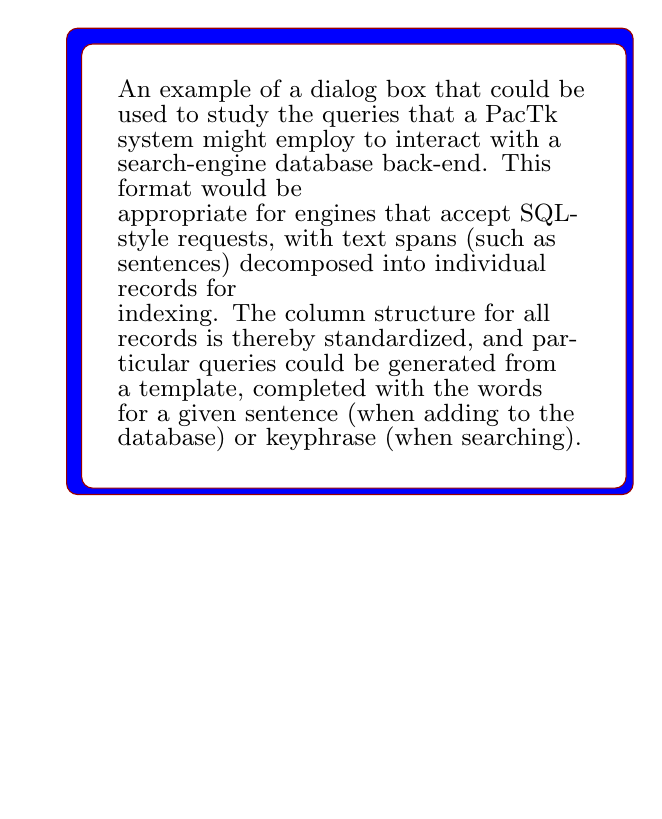
\begin{tikzpicture}

\node at (0,0) [text=white] {X};

\begin{scope}[transform canvas={scale=0.6, shift={(24.6,24.5)}},overlay]

\draw [rotate=20.9245, fill=white] (-1.5pt, 0pt) -- ++(up:5pt) -- ++(-5pt, -2pt) -- ++(6.5pt, 17pt)
                      -- ++(6.5pt, -17pt) -- ++(-5pt, 2pt) -- ++(down:5pt) -- cycle;

\end{scope}



\node [draw=red!60!black, fill=blue, anchor = south west, rounded corners,
text width=6cm, inner sep=17pt, xshift=-8pt, yshift=-8pt, font={\fontsize{9}{9}\selectfont}] (ltext)
(s1) at (.52, 3.8) {{
An example of a dialog box that could be used to study the 
queries that a PacTk system might employ to interact with a 
search-engine database back-end.  This format would be\\
appropriate for engines that accept SQL-style requests, 
with text spans (such as sentences) decomposed into 
individual records for\\indexing.  The column structure 
for all records is thereby standardized, and particular 
queries could be generated from a template, 
completed with the words for a given sentence 
(when adding to the database) or keyphrase 
(when searching).   
}
};


\node [draw=red!60!black, fill=white, anchor = south west, rounded corners,
text width=6cm, inner sep=13pt, font={\fontsize{9}{9}\selectfont}] (ltext-inner)
 at (.43, 3.6) {
An example of a dialog box that could be used to study the 
queries that a PacTk system might employ to interact with a 
search-engine database back-end.  This format would be\\ 
appropriate for engines that accept SQL-style requests, 
with text spans (such as sentences) decomposed into 
individual records for\\indexing.  The column structure 
for all records is thereby standardized, and particular 
queries could be generated from a template, 
completed with the words for a given sentence 
(when adding to the database) or keyphrase 
(when searching).
};





\end{tikzpicture}
}}

}\fi



\ifnum\value{page}=8{
\AtTextLowerLeft{\hspace{18pt}\raisebox{1pt}{

\begin{tikzpicture}

\node at (0,0) [text=black!7] {X};




\node [draw=red!60!black, fill=blue, anchor = south west, rounded corners,
text width=15cm, inner sep=17pt, xshift=-8pt, yshift=-8pt, font={\fontsize{9}{9}\selectfont}] (ltext)
 at (2.4, 11.9) {{Converting PDF files to SVG pages allows each page to 
have its own web address.  This enables publishers to organize pages 
into an online concordance indexed by topic or by annotated content.
}
};


\node [draw=red!60!black, fill=white, anchor = south west, rounded corners,
text width=15cm, inner sep=13pt, font={\fontsize{9}{9}\selectfont}] (ltext-outer)
 at (2.33, 11.84) {Converting PDF files to SVG pages allows each page to 
have its own web address.  This enables publishers to organize pages 
into an online concordance indexed by topic or by annotated content.
};





\node [draw=red!60!black, fill=blue, anchor = south west, rounded corners,
text width=18cm, inner sep=17pt, xshift=-8pt, yshift=-8pt, font={\fontsize{9}{9}\selectfont}] (ltext)
 at (.4, 4.2) {{In this case, a concordance was compiled by grouping pages 
into categories based on annotations.  The concordance was then 
published online as a master index, with links for each page presented 
alongside a checkbox-based table showing the category 
distribution per page.
}
};


\node [draw=red!60!black, fill=white, anchor = south west, rounded corners,
text width=18cm, inner sep=13pt, font={\fontsize{9}{9}\selectfont}] (ltext-inner)
 at (.33, 4.1) {In this case, a concordance was compiled by grouping pages 
into categories based on annotations.  The concordance was then 
published online as a master index, with links for each page presented 
alongside a checkbox-based table showing the category 
distribution per page.
};


\node [draw, rectangle, minimum width=165pt, minimum height=28pt, 
anchor = south west, rounded corners,
draw=teal!40!black] (s1) at (.7,.33) {};


\draw  [->,>=stealth', line width=4pt, draw=tp!50] ([yshift=14pt] s1.south east) to 
  [bend right=40, in=-90, out=-20] ([yshift=4pt, xshift=243pt] ltext.south) ;




\node [draw=red!60, fill=white, anchor = south west, rounded corners,
text width=4cm, inner sep=4pt, font={\fontsize{9}{9}\selectfont}] (stext)
 at (11.33, 1.6) {HTML columns were derived from a controlled vocabulary 
adopted for annotation text.
};

\draw  [--,>=stealth', line width=4pt, draw=tp!50] ([yshift=3pt, xshift=5pt] s1.south east) to 
   ([yshift=18pt, xshift=220] s1.south east) ;


\draw  [->,>=stealth', line width=4pt, draw=tp!50] ([yshift=18pt, xshift=218] s1.south east) to 
   ([yshift=3, xshift=20] stext.south) ;



\end{tikzpicture}
}}

}\fi




}

